\documentclass[12pt]{article}
\usepackage{fontspec} % 字型
\setmainfont{Taipei Sans TC Beta}
\usepackage{xeCJK} % 字型
\setCJKmainfont{Taipei Sans TC Beta}
\usepackage[top=1cm, bottom=1cm, left=1cm, right=1cm]{geometry} % 頁面設定
% \usepackage{indentfirst} % 首行縮排
\renewcommand{\baselinestretch}{1.5}
\pagenumbering{gobble} % 無頁碼
\usepackage{enumitem} % 列表縮排
\usepackage{zhnumber} % 中文數字
\usepackage{graphicx}
\usepackage{float}

\begin{document}

\section*{pA:STring}

\begin{itemize}[label={}, itemsep=0pt]
    \item 給你一個字串 $s$,重複執行以下的操作:刪除最左邊為\ "\textbf{ST}"\ 子字串,如果沒有就停止,並輸出剩餘字串的長度
    \item 測資範圍:$2 \leq \mid s \mid \leq 2 \times 10^5$,$\mid s \mid$ 為偶數,S 和 T 的數量相同
    \item \begin{center}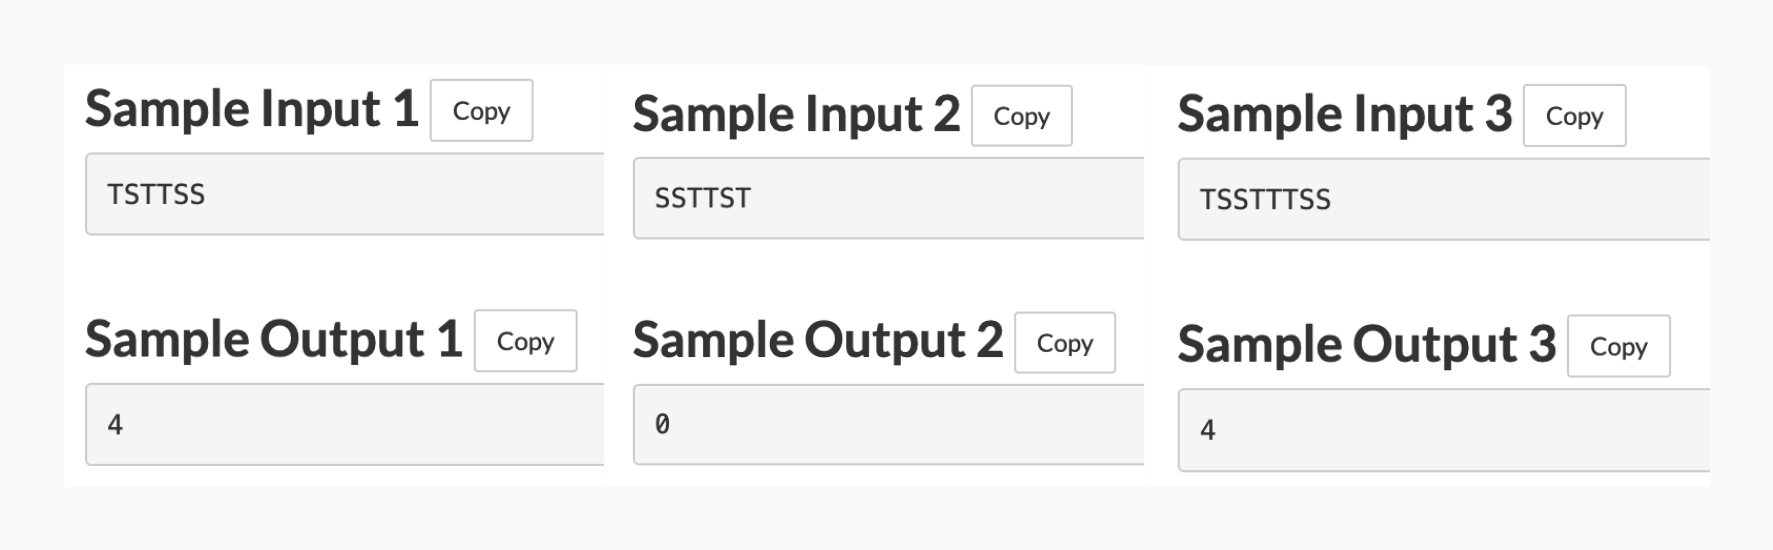
\includegraphics[width=18.0cm]{img/pA}\end{center}
\end{itemize}

\section*{pB:括號配對}

\begin{itemize}[label={}, itemsep=0pt]
    \item 給你一個字串 $s$,只由 <\ > (\ ) [\ ] \{\ \} 組成,左括號之間\textbf{可以互相替換},右括號同理,請判斷 $s$ 是否可以變成合法的括號序列,如果可以就\textbf{輸出最少的替換次數},否則輸出\ "\textbf{Impossible}"
    \item 測資範圍:$0 \leq \mid s \mid \leq 2 \times 10^6$
    \item \begin{center}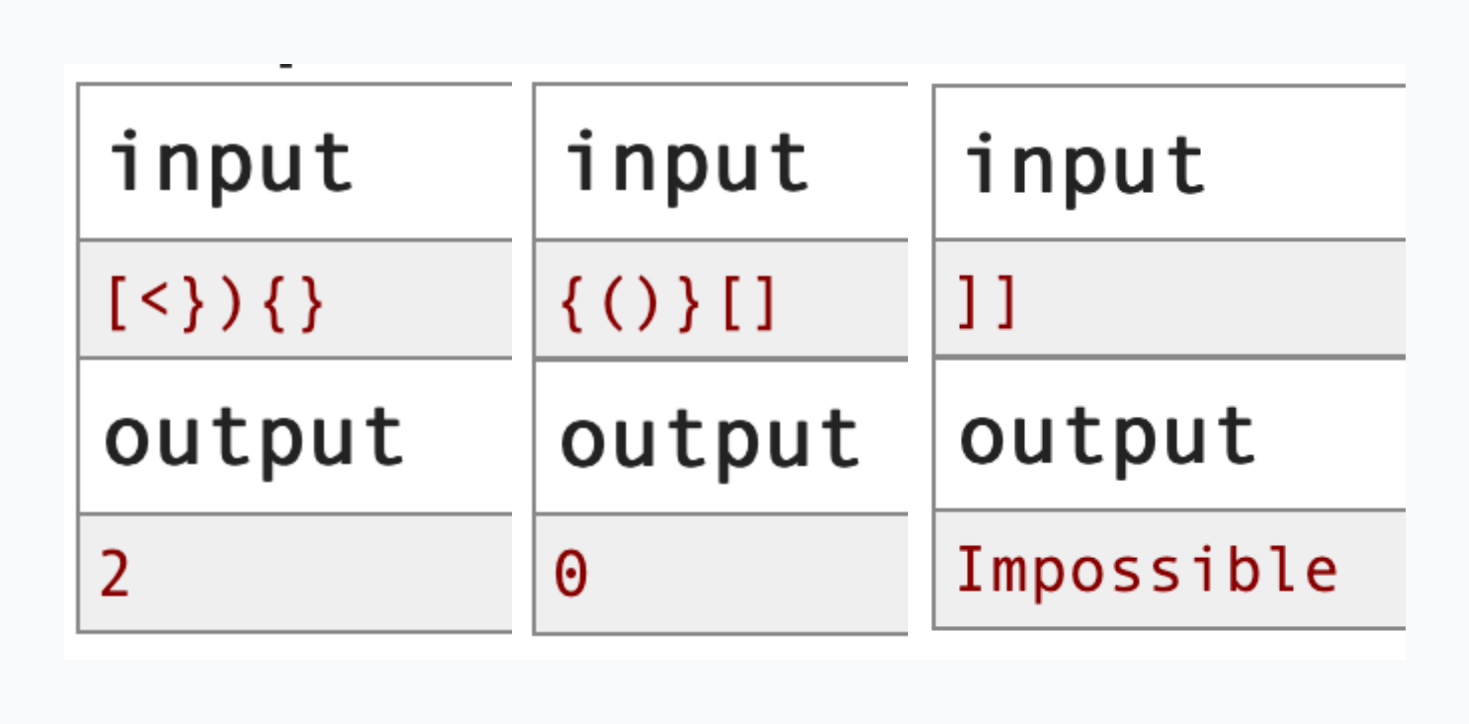
\includegraphics[width=10.0cm]{img/pB}\end{center}
\end{itemize}

\pagebreak

\section*{pC:最近較小數字}

\begin{itemize}[label={}, itemsep=0pt]
    \item 給你一個字串 $n$ 個數字 $a_i$(based-1),請對於每個 $a_i$ \textbf{在它左邊且比它小的最近位置}
    \item 測資範圍:$1 \leq n \leq 2 \times 10^5$,$1 \leq a_i \leq 10^9$
    \item \begin{center}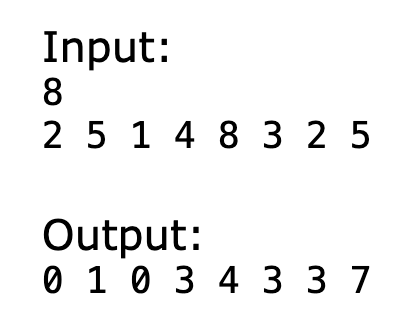
\includegraphics[width=6.0cm]{img/pC}\end{center}
\end{itemize}

\section*{pD:儲存站}

\begin{itemize}[label={}, itemsep=0pt]
    \item 有一個無限容量的儲存站,貨物\textbf{只會左進右出},並且\textbf{相對順序不會改變},接下來有 $q$ 個操作
    \begin{itemize}[label={-}, itemsep=0pt]
        \item $1\ x\ c$:把 $c$ 個價值為 $x$ 的貨物放進儲存站
        \item $2\ c$:把 $c$ 個貨物取出,並輸出貨物的總價價值
    \end{itemize}
    \item 測資範圍:$1 \leq q \leq 2 \times 10^5$,$0 \leq x \leq 10^9$,$1 \leq c \leq 10^9$
    \item \begin{center}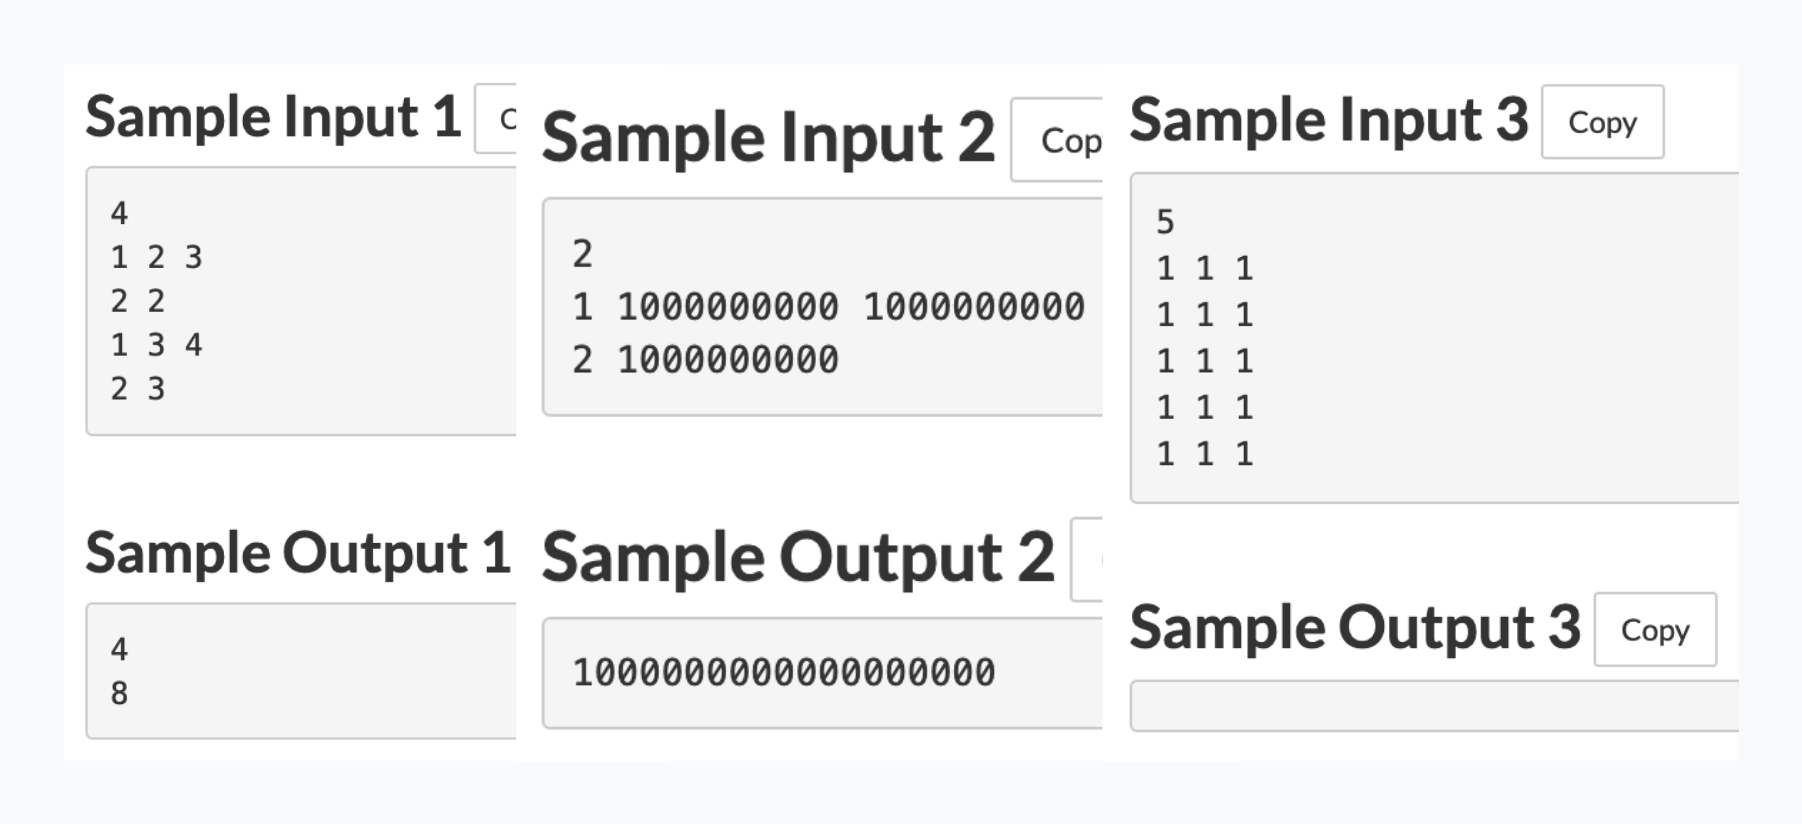
\includegraphics[width=18.0cm]{img/pD}\end{center}
\end{itemize}

\pagebreak

\section*{pE:LR 排列}

\begin{itemize}[label={}, itemsep=0pt]
    \item 你有一個字串 $s$,對於一個陣列 $V=\{0\}$,對於每個 $i$ 操作如下
    \begin{itemize}[label={-}, itemsep=0pt]
        \item $s_i = `L'$:把 $i$ 插入在 $i-1$ 的左邊
        \item $s_i = `R'$:把 $i$ 插入在 $i-1$ 的右邊
    \end{itemize}
    請輸出操作完後的陣列狀態
    \item 測資範圍:$1 \leq q \leq 5 \times 10^5$,$\mid s \mid = n$,$s$ 僅由 `L' 和 `R' 組成
    \item \begin{center}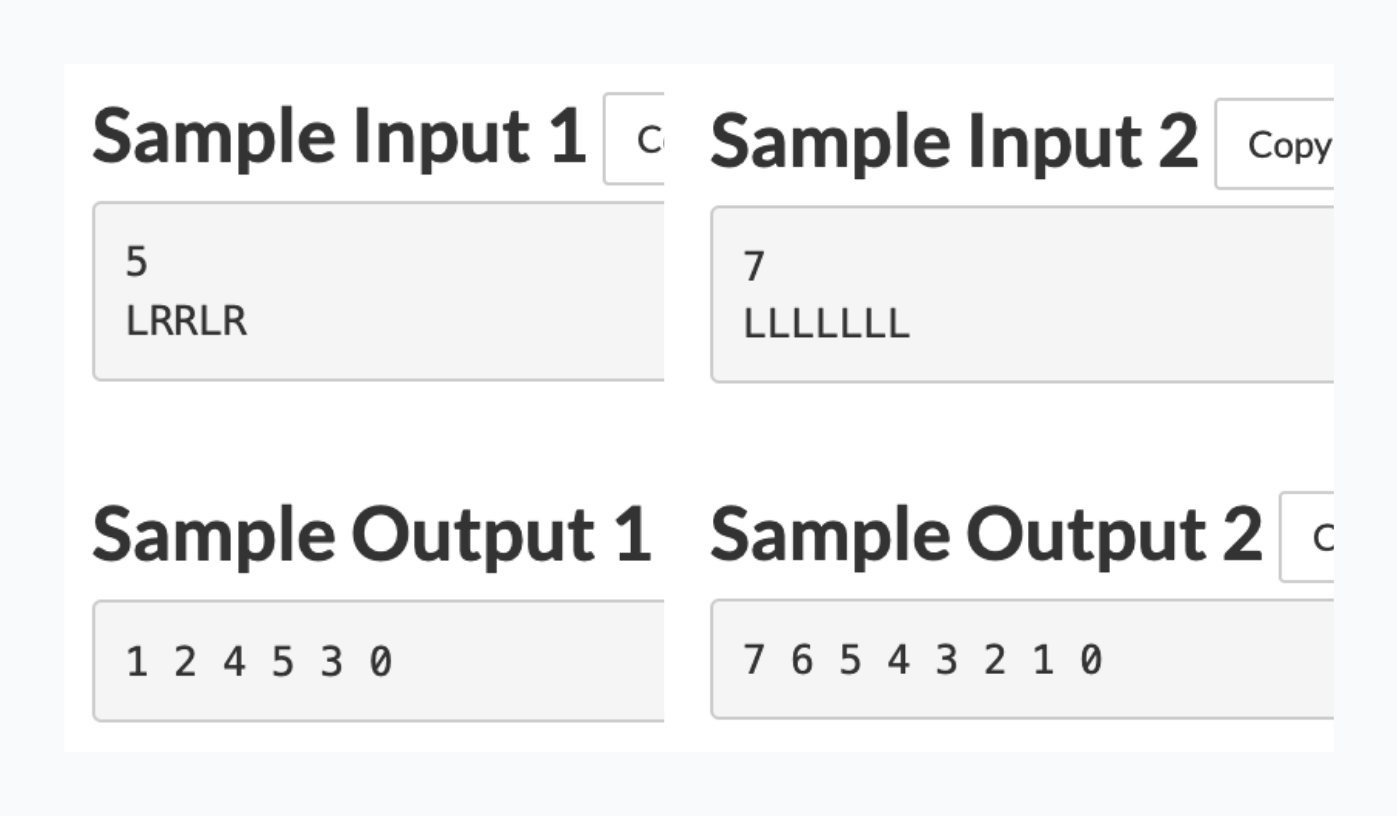
\includegraphics[width=13.0cm]{img/pE}\end{center}
\end{itemize}

\section*{pF:木棒組合}

\begin{itemize}[label={}, itemsep=0pt]
    \item 你有 $n$ 個總長為 $x$ 的木棍,每根木棍的長度為 $d_i$,兩個木棍\textbf{相連的成本為他們的長度和},請找出\textbf{最小的成本使得所有木棍相連}
    \item 測資範圍:$1 \leq x \leq 10^9$,$1 \leq n \leq 2 \times 10^5$,$\sum d_i = x$
    \item \begin{center}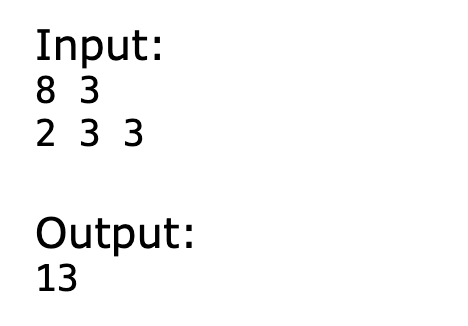
\includegraphics[width=6.0cm]{img/pF}\end{center}
\end{itemize}

\section*{pG:藤原千花與字串}

\begin{itemize}[label={}, itemsep=0pt]
    \item 千花有 $N$ 個字串 $s_i$ 依序紀錄,她想知道每次紀錄時\textbf{字典序不超過現在新寫的單詞裡字典序最大的單詞},請你對於每次紀錄輸出她想找的詞,如果沒有就輸出 -1。
    \item 測資範圍:$1 \leq N \leq 2 \times 10^5$,$1 \leq \mid s_i \mid \leq 10$
    \item \begin{center}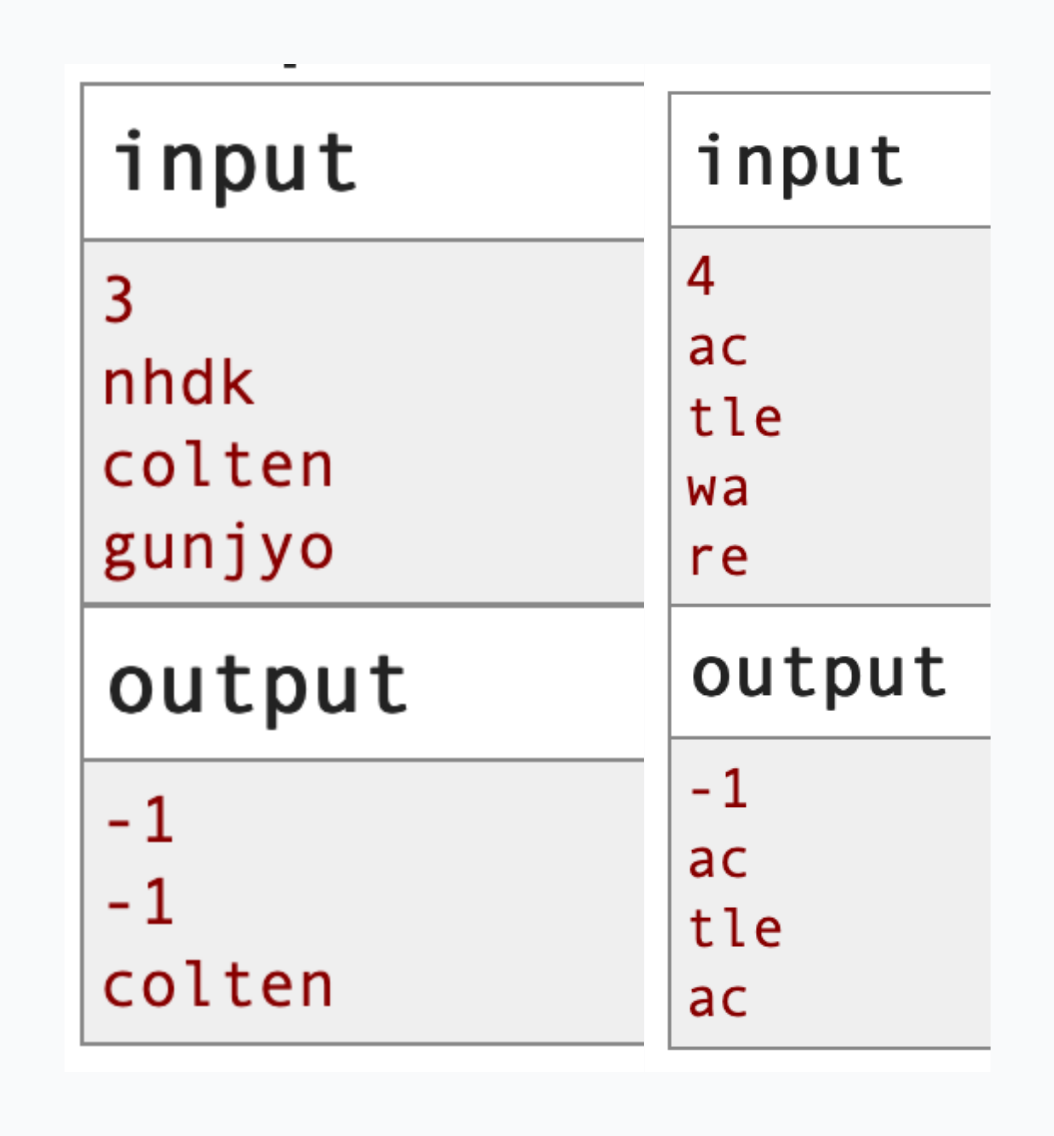
\includegraphics[width=5.0cm]{img/pG}\end{center}
\end{itemize}

\section*{pH:木棒切割}

\begin{itemize}[label={}, itemsep=0pt]
    \item 你有一個總長為 $L$ 公尺的木棍,木棍從左到右有 $1 \sim N-1$ 的標記,第 $i$ 個標記在離木棍左端 $i$ 公尺,對於接下來的 $Q$ 個查詢 $(c_i, x_i)$,操作如下
    \begin{itemize}[label={-}, itemsep=0pt]
        \item $c_i = 1$:在標記為 $x_i$ 的地方切一刀,將木棍分成兩半
        \item $c_i = 2$:輸出有標記為 $x_i$ 的木棍的長度
    \end{itemize}
    \item 測資範圍:$1 \leq L \leq 10^9$,$1 \leq Q \leq 2 \times 10^5$,$c_i = \{1, 2\}$\\
    \hspace*{5em} $1 \leq x_i \leq N-1$,不會切割已經切割過的地方,不會查詢已經被切割的標記
    \item \begin{center}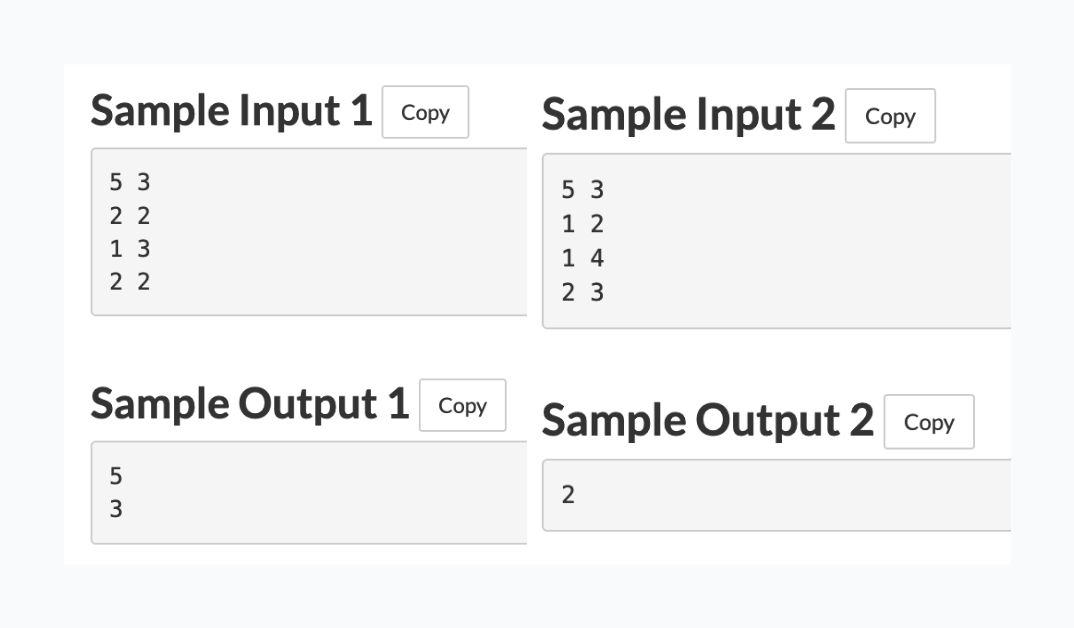
\includegraphics[width=12.0cm]{img/pH}\end{center}
\end{itemize}

\section*{pI:演唱會門票}

\begin{itemize}[label={}, itemsep=0pt]
    \item 你有 $n$ 張演唱會門票價格為 $h_i$,會有 $m$ 個人依序購買門票,它們各自的最高花費為 $t_i$,對於每個人你要賣出他們可以買的最高價門票,請\textbf{輸出每個人拿到的門票價格},如果他沒辦法買到票的話就輸出 -1
    \item 測資範圍:$1 \leq n, m \leq 2 \times 10^5$,$1 \leq h_i, t_i \leq 10^9$
    \item \begin{center}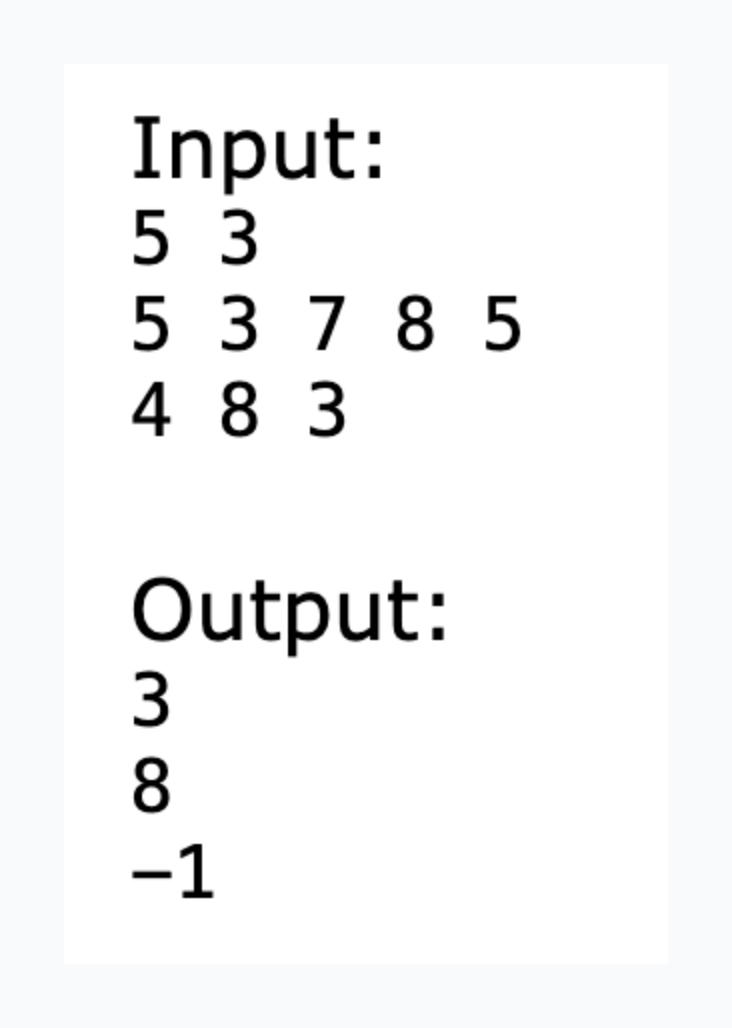
\includegraphics[width=4.0cm]{img/pI}\end{center}
\end{itemize}

\section*{pJ:新增資料夾(1)}
\begin{itemize}[label={}, itemsep=0pt]
    \item 你有 $N$ 個新增資料夾的操作,每個資料夾的名字為 $S_i$。對於第 $i$ 個操作,如果前面已經創建名字同為 $S_i$ 的資料夾,則此資料夾會叫做 $S_i(X)$($X$ 為 $S_i$ 出現過的次數),否則是原本的名稱
    \item 測資範圍:$1 \leq N \leq 2 \times 10^5$
    \item \begin{center}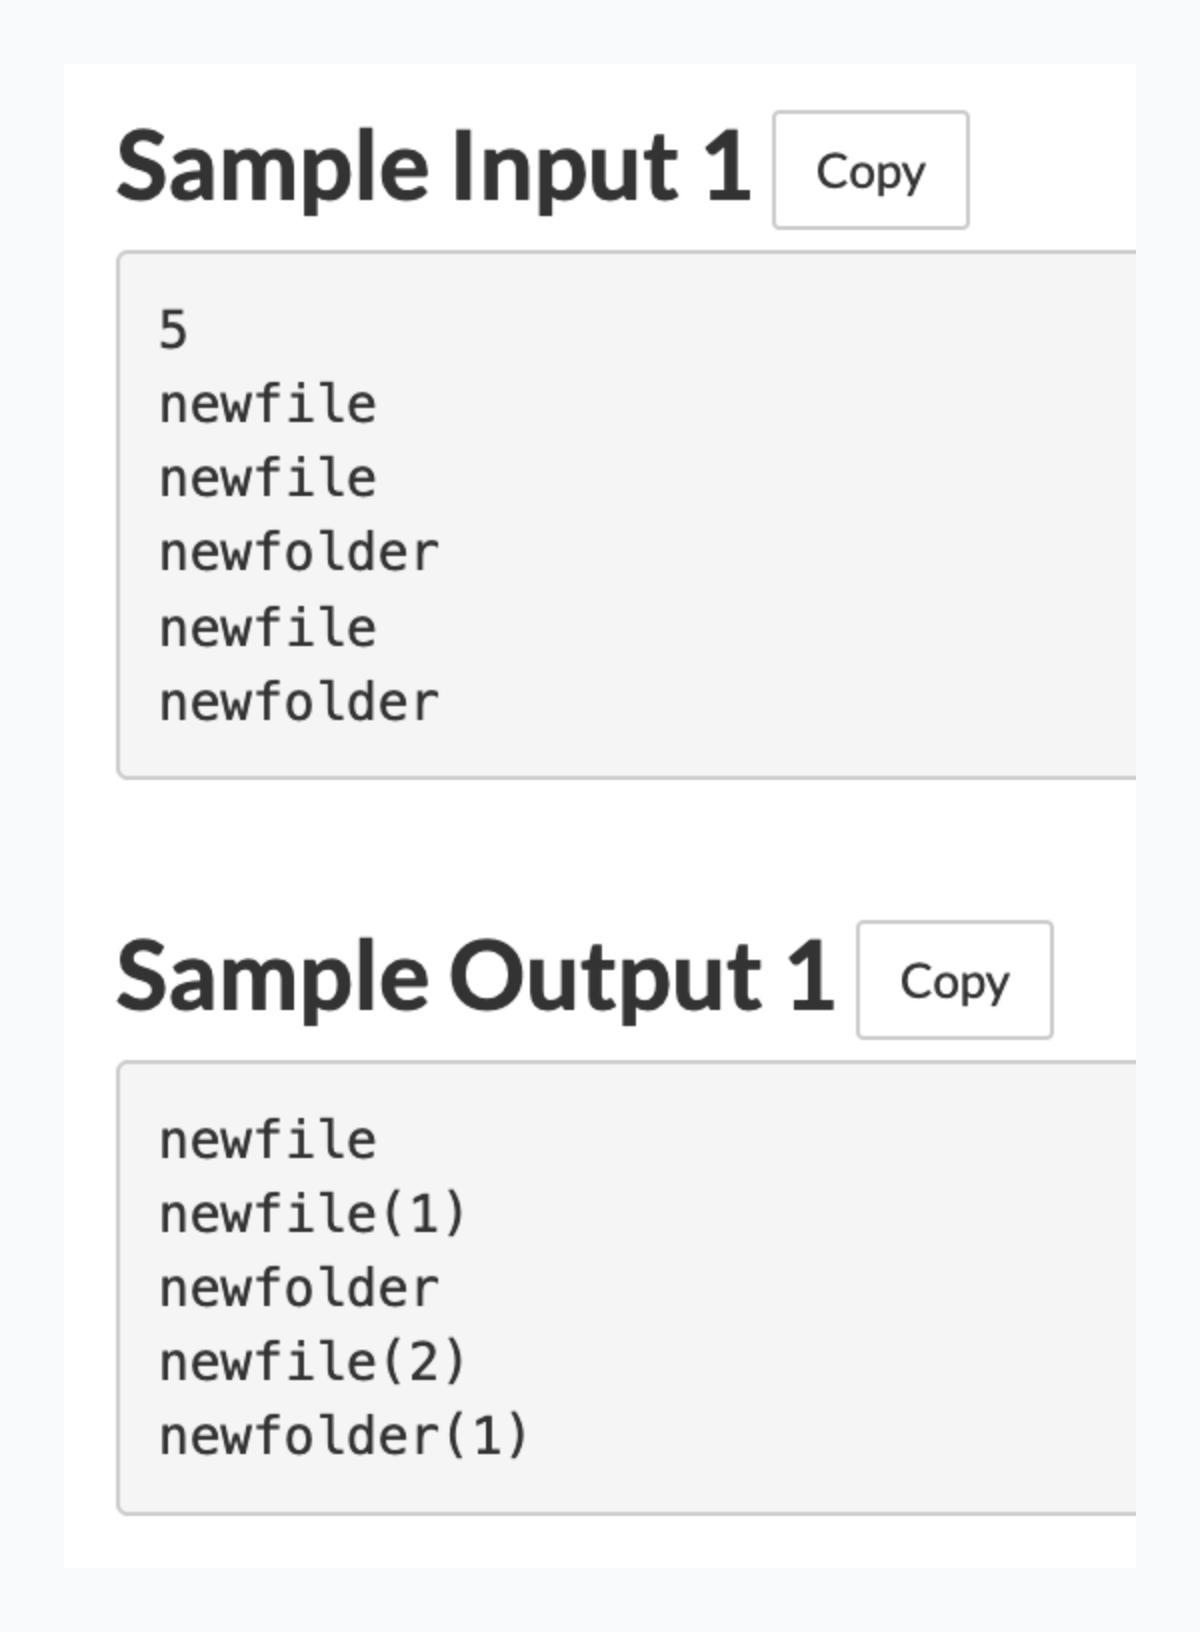
\includegraphics[width=7.0cm]{img/pJ}\end{center}
\end{itemize}
\end{document}